\section{Scalably Feasible QoI Regions}
\label{sec:scal_feasible_qoi}

Now let us consider a special case where nodes collect a total of $k_{req}$ images, but each image must come from a different node, perhaps because each node only has one image or maybe by design to provide increased credibility through corroboration, another contextual metric of interest in QoI-aware networks. This scenario allows us to illustrate an interesting observation.  

Consider a set of QoI requirements that include completeness and timeliness, $\mathbf{q} = \{C,T\}$.  As previously noted, a certain number of images are required to achieve this desired level of completeness, $Q(C) = k_{req}$.  Unlike the model used in Section \ref{sec:network_design}, however, each node can contribute only one image to $k_{req}$, which implies a minimum network size of $N \geq k_{req}$ in order to achieve the completeness outlined in the QoI requirements.  On the other hand, applying the framework of Section \ref{sec:qoi_scalability} to this network, we can determine the maximum network size, which we will call $N_{max}$ here for distinction.  

These two facts are important, because when $N_{max} < k_{req}$, then it is not possible to provide the QoI level $\mathbf{q}$.  Hence, this set of QoI requirements is infeasible, or \emph{scalably infeasible}.  This phenomenon defines the concept of a \emph{Scalably Feasible QoI Region}, which refers to the region in which all sets of QoI pairs can be supported with the given network signature.  

\vspace{-3mm}
\begin{figure}[ht]
\centering
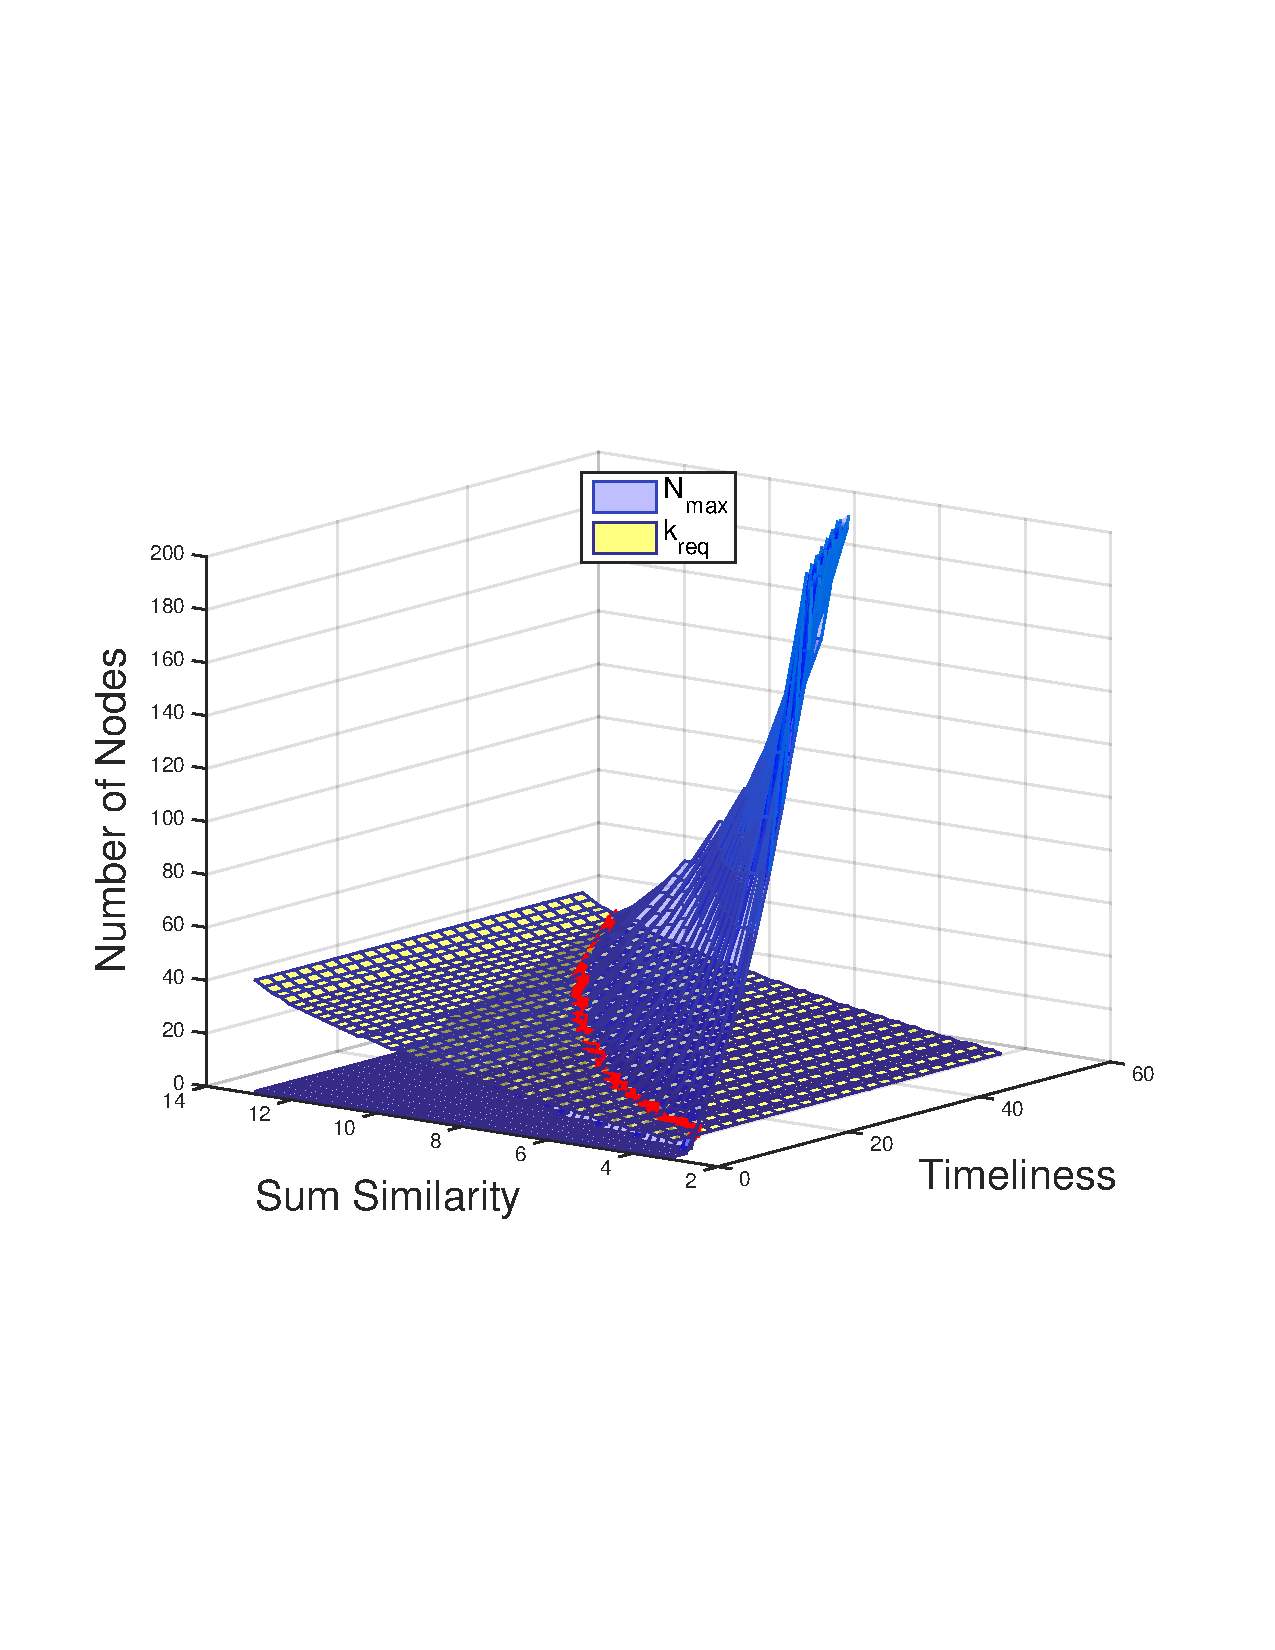
\includegraphics[scale=0.31, clip=true, trim=10mm 65mm 20mm 77mm]{figures/scal_feas_qoi/scal_feas_qoi_region_3d_plot_3.pdf}
\vspace{-3mm}
\caption{The blue plane represents maximum scalability, and the yellow plane represents minimum required images.  Therefore, all (Sum Sim., Timeliness) pairs to the right of the red line are within the scalably feasible QoI region.}
 \label{fig:scal_feasible_region}
 \vspace{-3mm}
\end{figure}

Figure \ref{fig:scal_feasible_region} provides a visual representation of this region for a grid network that institutes the given traffic model assuming traffic is routed over randomly chosen shortest-path routes.
%\footnote{Details of applying the framework are omitted due to space constraints.}.  
Here, $N_{max}$, calculated for $\mathbf{q}$ pairs from $\{2.5,1\}$ to $\{13.0, 50\}$, is shown in the graph by the blue surface.  On the same graph is the number of images required, $k_{req}$, for each Sum Similarity requirement, shown with the yellow surface on the graph.  The intersection of these two surfaces, displayed with a red line, provides the edge of the scalably feasible QoI region.  In this example, all sum QoI pairs to the right of this line, i.e. the region where $N_{max} > k_{req}$, are scalably feasible.  

In general, regardless of how many images a node has, it is possible to analyze the trade-off between different QoI attributes for a fixed value of maximum network size, $N_{max}$.  Specifically, by fixing $N$ in Table \ref{table:scal_eqs},
%(\ref{eq:clique_gen})-(\ref{eq:grid_gen}), 
one can obtain $T$ and $k_{req}$ (and, hence, $C$) resulting in the set of supportable $\{C,T\}$ pairs defining a feasible region for QoI. This region can be visualized by intersecting the blue scalability curve with a flat surface fixed at $N_{max}$ instead of the yellow surface in Figure \ref{fig:scal_feasible_region}.  The scenario given in this section goes one step further and also takes into account  the network size actually required to generate/support a given QoI requirement (using the non-flat yellow surface derived from experimental results in Figure \ref{fig:scal_feasible_region}).
